\newif\ifPDF%
\newif\ifBNPDF%
\PDFtrue
%\BNPDFtrue

% referencias
\addbibresource{./files/gbTeXbib-7moCongresoMKT.bib}

\ifPDF
% control de inconsistencias de principio y fin de linea
\usepackage[hyphenation,draft,homeoarchy,homeoarchywordcolor=orange,homeoarchycharcolor=yellow]{impnattypo}
\usepackage[allcolors=blue,colorlinks,unicode]{hyperref}
\usepackage{easyReview}
\usepackage{hyperxmp}
\hypersetup{
pdfauthor={Alberto Moyano},
pdfsubject={-},
pdfauthortitle={Editor},
pdfdate={2024-11},
pdfcaptionwriter={Alberto Moyano},
pdfkeywords={-},
pdftitle={-},
pdfcreator={gbTeXpublisher},
pdfproducer={Ecosistema de LaTeX},
unicode=true,
bookmarks=true,
pdfdisplaydoctitle=true,
pdfnewwindow=true
}

	\else
	\ifBNPDF
	\usepackage[hidelinks,unicode]{hyperref}
	\usepackage{easyReview}
	\usepackage{hyperxmp}
	\hypersetup{
pdfauthor={Alberto Moyano},
pdfsubject={-},
pdfauthortitle={Editor},
pdfdate={2024-11},
pdfcaptionwriter={Alberto Moyano},
pdfkeywords={-},
pdftitle={-},
pdfcreator={gbTeXpublisher},
pdfproducer={Ecosistema de LaTeX},
unicode=true,
bookmarks=true,
pdfdisplaydoctitle=true,
pdfnewwindow=true
}

	\fi
\fi


\usepackage{chemfig}
\usepackage{amsmath}
\usepackage{tikz}
\begin{document}
\frontmatter

% página 1
\newpage
\thispagestyle{empty}
{\textcolor{white}{.}}

% página 2
\newpage
\thispagestyle{empty}
{\textcolor{white}{.}}

% página 3
\newpage
\thispagestyle{empty}
{\textcolor{white}{.}}

\vspace{30mm}

\begin{center}
	\LARGE{<título>}
\end{center}

% página 4
\newpage
\thispagestyle{empty}
{\textcolor{white}{.}}

% página 5
\newpage
\thispagestyle{empty}
\begin{center}%,draft
{\sc\large{nombre de autor}}\\ %compiladoras
\end{center}

\vspace{30mm}

\begin{center}
\LARGE{título}\\\vspace{10mm}

\Large{subtítulo}
\end{center}

\vfill

\begin{figure}[b]
\centering
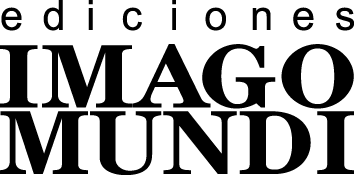
\includegraphics[width=20mm]{./media/logo-imago-ByW.png}
\end{figure}

% página 6
\newpage
\thispagestyle{empty}
\begin{figure}[t]
\centering
\vspace{-10mm}

\includegraphics[width=20mm]{./media/desconocido.png}\\
\end{figure}

\noindent autor \\
\noindent título. 1a ed. Buenos Aires: 2023.\\
\noindent 000 p.; 15.5x23 cm. ISBN 978-950-793-000-0 \\
\noindent 1. \\
\noindent CDD .\\
\noindent Fecha de catalogación: 00/00/20xx \\
\noindent \textcopyright~20xx, autor \\
\noindent \textcopyright~20xx, Ediciones Imago Mundi\\
\noindent Imagen de tapa: .\\
\noindent Hecho el depósito que marca la ley 11.723\\
\noindent Impreso en Argentina, tirada de esta edición: 000 ejemplares\\

\vfill

\noindent Ninguna parte de esta publicación, incluido el diseño de cubierta, puede ser reproducida, almacenada o transmitida de manera alguna ni por ningún medio, ya sea eléctrico, químico, mecánico, óptico, de grabación o de fotocopia, sin permiso previo por escrito del editor. Este libro se terminó de imprimir en el mes de xxxx de 20xx en San Carlos Impresiones, Virrey Liniers 2203, Ciudad Autónoma de Buenos Aires, República Argentina.


% pagina dedicatoria, si va como epígrafe habilitar este segmento de código
\cleardoublepage
\thispagestyle{empty}
{\textcolor{white}{.}}
\vspace{40mm}
\epigraph{<va texto>.}{}
\cleardoublepage

% si va como capítulo, habilitar este otro


\Author{Sumario}
\tableofcontents

\chapter[\hspace{2pc}Agradecimiento a Donald Knuth]{Agradecimiento a Donald Knuth}
\Author{Alberto Moyano}

Este libro no podría comenzar sin expresar nuestro más sincero agradecimiento a uno de los pioneros más influyentes en el campo de la informática: el profesor Donald E. Knuth. Su legado ha dejado una huella indeleble en la historia de la ciencia computacional, y su contribución va mucho más allá de los límites del software y las matemáticas. Este prólogo es un tributo a su extraordinaria carrera y a su trabajo monumental, en particular a la creación de \TeX{}, el sistema tipográfico que ha revolucionado la manera en que preparamos documentos técnicos, científicos y académicos.

El nombre de Knuth está íntimamente asociado con la obra maestra \citetitle{@5288-DONALD1968}, una serie de volúmenes que sigue siendo la referencia definitiva en el campo de la algoritmia y las estructuras de datos. Sin embargo, uno de sus aportes más significativos a la comunidad académica es la creación de \TeX{}, un sistema diseñado para permitir la producción de textos con calidad tipográfica profesional. Su diseño no solo es un testimonio de su genio matemático, sino también de su amor por la tipografía.

Es importante reconocer que \TeX{} surgió como una solución a un problema personal que Knuth enfrentó mientras escribía el segundo volumen de su serie. Insatisfecho con la calidad de impresión de las fórmulas matemáticas en su libro, decidió tomar cartas en el asunto y crear un sistema que permitiera a los matemáticos, científicos y académicos preparar documentos con una presentación impecable. \TeX{} ha sido adoptado de manera global en la comunidad académica, especialmente en matemáticas, física y ciencias de la computación, debido a su capacidad para manejar con precisión la complejidad de las notaciones matemáticas.

No obstante, uno de los derivados más conocidos de \TeX{} es \LaTeX{}, un sistema de macros desarrollado por Leslie Lamport, que simplifica el uso de \TeX{} y lo hace accesible a un público más amplio. \LaTeX{} ha sido una herramienta invaluable para investigadores, estudiantes y profesionales que desean preparar documentos complejos de manera eficiente y con un control riguroso sobre el diseño tipográfico. Aunque Lamport fue responsable de su creación, es el trabajo de Knuth en \TeX{} lo que establece la base sobre la cual \LaTeX{} ha florecido.

Knuth ha sido un defensor de los principios de precisión, elegancia y eficiencia en el diseño de software, y sus enseñanzas han inspirado a generaciones de científicos computacionales. Además, su enfoque hacia la corrección de errores es otro aspecto a destacar. A lo largo de su carrera, ha ofrecido recompensas a quienes encontraran errores en su código o en sus libros, un gesto que refuerza su compromiso con la excelencia y la mejora continua.

En resumen, el impacto de Donald Knuth en la informática moderna es inconmensurable. Su trabajo en \TeX{} y sus contribuciones a la ciencia de la computación continúan mejorando la vida de quienes trabajan en el mundo académico y científico. Este documento es un pequeño testimonio de gratitud por sus contribuciones, que han sido fundamentales para el desarrollo de herramientas que, como este artículo, nos permiten comunicar nuestras ideas de manera clara y profesional.

Gracias, profesor Knuth, por su visión, por su pasión y por su dedicación a la excelencia. Su legado sigue vivo en cada línea de código que escribimos, en cada fórmula matemática que tipografiamos y en cada libro que editamos con \TeX{} y \LaTeX{}.


%\input{./artcap/prologo.tex}

\mainmatter

%\chapter{Crecimiento poblacional en el planeta}

\section{Introducción}

El crecimiento poblacional es uno de los fenómenos más importantes que enfrenta la humanidad en el siglo XXI. Desde la revolución industrial, la población mundial ha experimentado un crecimiento exponencial, impulsado por avances en la medicina, la tecnología y la agricultura. Sin embargo, este aumento de la población también plantea desafíos importantes en términos de sostenibilidad ambiental, recursos naturales y políticas públicas.

\begin{imagen}[h!]
	\centering
	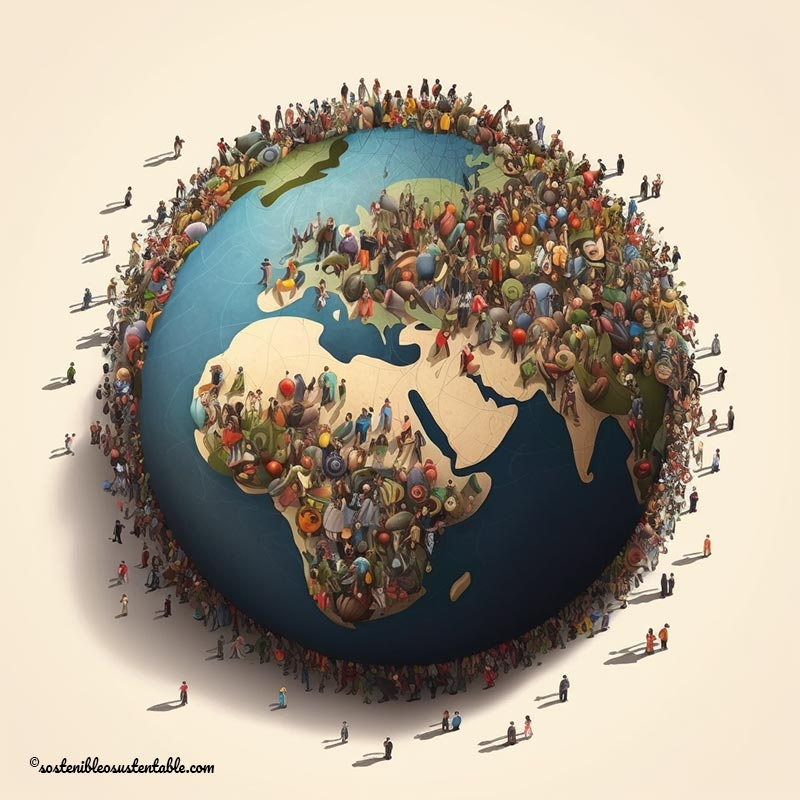
\includegraphics[width=\textwidth]{./media/people.jpg}
	\caption{}
\end{imagen}

En este capítulo se explorarán las tendencias de crecimiento poblacional a nivel mundial y se analizarán las consecuencias sociales y económicas derivadas de este fenómeno. Se utilizarán datos y ejemplos de diferentes regiones del mundo para ilustrar los cambios demográficos recientes.

\section{Tendencias globales}

A lo largo de los siglos, la población mundial ha crecido de manera desigual. La mayoría del crecimiento poblacional se ha concentrado en países en desarrollo, mientras que muchos países desarrollados han experimentado una desaceleración en sus tasas de crecimiento, e incluso, en algunos casos, un decrecimiento.

\subsection{Cifras del crecimiento poblacional}

El cuadro~\ref{cuadro1} muestra la evolución de la población mundial en las últimas décadas, así como las proyecciones futuras para el crecimiento poblacional.

\begin{table}[!ht]
\sf\footnotesize\setlength\tabcolsep{4pt}
\centering
\begin{tabular}{l | cccc}
\toprule
& \textbf{Población & \textbf{Tasa de crecimiento} & \textbf{Esperanza de vida} & \textbf{Población urbana} \\
\textbf{Año} & \textbf{(miles de millones)} & \textbf{(\%)} & \textbf{(años)} & \textbf{(\%)} \\
\midrule
1950 & 2.5 & 1.8 & 48 & 30 \\
\midrule
1980 & 4.4 & 2.1 & 60 & 39 \\
\midrule
2010 & 6.9 & 1.2 & 70 & 51 \\
\midrule
2023 & 8.0 & 1.0 & 72 & 56 \\
\midrule
2050* & 9.7 & 0.8 & 77 & 68\\
\bottomrule
\end{tabular}
\caption{Crecimiento poblacional mundial y proyecciones futuras (*proyecciones).}
\label{cuadro1}
\end{table}

En el cuadro~\ref{cuadro1} se observa cómo la tasa de crecimiento poblacional ha disminuido, mientras que la esperanza de vida y la urbanización han ido en aumento. Las proyecciones indican que la población mundial alcanzará los 9.7 mil millones para 2050, aunque con una tasa de crecimiento más baja que en décadas anteriores.

\section{Factores que afectan el crecimiento poblacional}

El crecimiento de la población está influenciado por varios factores. Entre los más importantes se encuentran las tasas de natalidad, las tasas de mortalidad y las políticas migratorias. A continuación, se presentan algunos de los factores clave que influyen en las dinámicas poblacionales globales.

\begin{table}[!ht]
\sf\footnotesize\setlength\tabcolsep{4pt}
\centering
\begin{tabular}{>{\raggedright\arraybackslash}m{3.4cm} | >{\raggedright\arraybackslash}m{7cm}}
\toprule
\textbf{Factor} & \textbf{Descripción}\\
\midrule
Tasa de natalidad & Cantidad de nacimientos por cada \num{1000} habitantes en un año. \\
\midrule
Tasa de mortalidad & Cantidad de muertes por cada \num{1000} habitantes en un año. \\
\midrule
Esperanza de vida & Número promedio de años que se espera que viva una persona al nacer, influida por factores como la salud y la economía. \\
\midrule
Migración & Movimiento de personas entre regiones, que puede aumentar o disminuir la población de un país o región. \\
\midrule
Políticas gubernamentales & Las políticas de planificación familiar y los incentivos económicos influyen en las tasas de natalidad y mortalidad. \\
\midrule
Condiciones económicas & El crecimiento económico suele estar asociado con una disminución en las tasas de natalidad y mortalidad. \\
\bottomrule
\end{tabular}
\caption{Factores que influyen en el crecimiento poblacional.}
\label{tabla2}
\end{table}

\subsection{Tendencias regionales}

El crecimiento poblacional es especialmente pronunciado en regiones como África subsahariana, donde las tasas de natalidad siguen siendo altas. Sin embargo, en muchas regiones de Europa y Asia Oriental, las tasas de natalidad han caído por debajo del nivel de reemplazo, lo que plantea preocupaciones sobre el envejecimiento de la población y la sostenibilidad de los sistemas de pensiones.

\section{Impacto social y económico}

El crecimiento poblacional tiene efectos significativos en las sociedades y las economías. El rápido aumento de la población puede ejercer presión sobre los recursos naturales, los sistemas de salud, la educación y el empleo. A su vez, un decrecimiento de la población o un envejecimiento significativo puede llevar a la escasez de mano de obra y problemas para mantener el sistema de pensiones.

Los países en desarrollo, con altas tasas de crecimiento, a menudo enfrentan desafíos relacionados con la sostenibilidad de sus recursos. Por otro lado, los países desarrollados que experimentan una disminución en el crecimiento poblacional, deben abordar los problemas del envejecimiento y la escasez de fuerza laboral.

\section{Conclusión}

El crecimiento poblacional es un tema de gran relevancia en la actualidad, con implicaciones profundas para el desarrollo económico y social de las naciones. A medida que la población mundial sigue creciendo, los desafíos de sostenibilidad, planificación urbana y uso de recursos naturales se vuelven más urgentes. Sin embargo, las proyecciones también indican una desaceleración de la tasa de crecimiento, lo que abre una ventana de oportunidad para abordar estos problemas de manera más efectiva.

El análisis de los factores que influyen en el crecimiento poblacional y las variaciones entre regiones nos permite entender mejor las dinámicas demográficas y planificar para un futuro más sostenible.

%	\begin{thebibliography}{9}
%
%		\bibitem{UN2019}
%		United Nations Department of Economic and Social Affairs.
%		\textit{World Population Prospects 2019: Highlights}.
%		United Nations, 2019.
%
%		\bibitem{WorldBank2021}
%		World Bank.
%		\textit{World Development Indicators: Population Dynamics}.
%		World Bank, 2021.
%
%	\end{thebibliography}

%ciencias sociales
\chapter{¿Por qué sube y baja la bolsa de valores?}

\section{Introducción}

La bolsa de valores es uno de los mercados financieros más importantes y a menudo genera una gran cantidad de incertidumbre y especulación. Los precios de las acciones y otros activos financieros suben y bajan debido a múltiples factores \parencite{@5287-FREDERIC2018,@5286-ZVI2013}. En este artículo, analizaremos algunos de los principales factores que afectan el movimiento de la bolsa y presentaremos una explicación económica de estos movimientos. Utilizaremos fórmulas económicas y un diagrama para ilustrar los conceptos clave.

\section{Factores que afectan la bolsa de valores}

Los precios en la bolsa de valores están influenciados por factores tanto macroeconómicos como microeconómicos. Los más importantes incluyen:

\begin{itemize}
\item \textbf{Noticias económicas}: informes de inflación, tasas de interés y crecimiento económico afectan las expectativas de los inversionistas.
\item \textbf{Política monetaria}: las decisiones del banco central sobre las tasas de interés influyen directamente en el costo de capital y las expectativas de los rendimientos.
\item \textbf{Resultados empresariales}: los ingresos y utilidades reportados por las empresas influyen en la percepción del valor de sus acciones.
\end{itemize}

\section{Modelo del precio de las acciones}

El valor de una acción puede ser modelado utilizando el enfoque de los flujos de caja descontados (\textit{Discounted Cash Flow, DCF}). El precio de una acción $P_0$ puede expresarse como la suma de los dividendos futuros esperados $D_t$, descontados a una tasa de descuento $r$, que representa el riesgo del activo:

\begin{equation}
P_0 = \sum_{t=1}^{\infty} \frac{D_t}{(1 + r)^t}
\end{equation}

Este modelo sugiere que los precios de las acciones subirán si los dividendos futuros esperados aumentan o si la tasa de descuento disminuye. Por el contrario, los precios bajarán si las expectativas de dividendos disminuyen o si la tasa de descuento aumenta.

\section{Oferta y demanda en el mercado}

El precio de una acción está determinado por la oferta y la demanda en el mercado de valores. Si la demanda de una acción supera la oferta, su precio subirá, y si la oferta supera la demanda, el precio caerá. Esto se puede modelar matemáticamente mediante una función de demanda:

\begin{equation}
Q_d = f(P, I, r)
\end{equation}

Donde:
\begin{itemize}
\item $Q_d$ es la cantidad demandada de acciones.
\item $P$ es el precio de la acción.
\item $I$ es el ingreso de los inversionistas.
\item $r$ es la tasa de interés.
\end{itemize}

De manera similar, la cantidad ofertada de acciones $Q_s$ está influenciada por factores como la liquidez y el número de acciones disponibles.

\section{Diagrama de la dinámica del mercado}

A continuación se presenta un diagrama simplificado utilizando TikZ, que muestra cómo interactúan la oferta y la demanda en el mercado de valores:

\begin{figure}[h!]
\centering
\begin{tikzpicture}
% Ejes
\draw[->] (0,0) -- (5,0) node[right] {Cantidad};
\draw[->] (0,0) -- (0,5) node[above] {Precio};

% Curva de demanda
\draw[thick] (0.5,4) .. controls (2,2) .. (4,0.5) node[right] {Demanda};

% Curva de oferta
\draw[thick] (0.5,0.5) .. controls (2,2) .. (4,4) node[right] {Oferta};

% Punto de equilibrio
\draw[dashed] (2.5,2.5) -- (2.5,0) node[below] {$Q^*$};
\draw[dashed] (2.5,2.5) -- (0,2.5) node[left] {$P^*$};

% Etiqueta de equilibrio
\node at (2.7,2.7) {Equilibrio};
\end{tikzpicture}
\caption{Interacción de la oferta y la demanda en el mercado de valores.}
\end{figure}

En este gráfico, el punto de equilibrio $(Q^*, P^*)$ representa el precio y la cantidad donde la oferta y la demanda se igualan. Si ocurre un cambio en alguno de los factores determinantes de la demanda o la oferta, el punto de equilibrio se desplazará, afectando el precio de las acciones.

\section{Factores adicionales}

Además de la oferta y la demanda, otros factores juegan un papel importante en los movimientos de la bolsa:

\subsection{Política monetaria y fiscal}
Las tasas de interés son un factor crucial en la valoración de activos financieros. Según el modelo CAPM (Capital Asset Pricing Model), el retorno esperado de un activo financiero $E(R_i)$ se calcula como:

\begin{equation}
E(R_i) = R_f + \beta_i (E(R_m) - R_f)
\end{equation}

Donde:
\begin{itemize}
\item $R_f$ es la tasa libre de riesgo.
\item $\beta_i$ es la sensibilidad del activo $i$ respecto al mercado.
\item $E(R_m)$ es el retorno esperado del mercado.
\end{itemize}

Este modelo indica que si la tasa libre de riesgo \(R_f\) aumenta, el retorno esperado de las acciones también aumentará, lo que puede provocar una caída en los precios actuales de las acciones debido a que los inversionistas exigen mayores rendimientos.

\subsection{Expectativas del mercado}

Las expectativas de los inversionistas sobre el futuro son otro factor clave que afecta el precio de las acciones. Los cambios en las expectativas pueden deberse a informes económicos, cambios en la política gubernamental o eventos inesperados como crisis económicas o avances tecnológicos.

\section{Conclusión}

El precio de las acciones en la bolsa de valores está determinado por una compleja interacción de factores económicos y psicológicos. Las fórmulas de valoración financiera, como el modelo de flujos de caja descontados y el CAPM, nos brindan herramientas para entender cómo la información disponible y las expectativas futuras influyen en los movimientos del mercado. Sin embargo, dado que los mercados financieros también están sujetos a la especulación y al comportamiento de los inversionistas, siempre existe un grado de incertidumbre asociado a los movimientos de la bolsa.
%finanzas, economía
\chapter{Análisis estructural de una viga trapezoidal}

\section{Introducción}

En el diseño de estructuras, las vigas son elementos fundamentales que soportan cargas a través de una distribución eficiente del material en su sección transversal. Una de las formas geométricas utilizadas en este contexto es la sección trapezoidal, la cual presenta ventajas tanto en términos de resistencia como de rigidez. Este artículo analiza las propiedades geométricas y mecánicas de una viga trapezoidal, destacando su momento de inercia, su comportamiento bajo cargas distribuidas y su aplicación en diversas estructuras.

A continuación, se presenta la figura de una viga trapezoidal. Las bases $b_1$ y $b_2$ representan los extremos inferior y superior de la viga, mientras que $s$ es la altura de la sección. El parámetro $x$ denota la longitud total de la viga, variando desde $x=0$ hasta $x=l$.

\begin{center}
\begin{tikzpicture}
% general shift to north east
\coordinate (O) at (0.5,0.5);
\draw[semithick] (0,0) -- (4,1); % bottom line in front
\draw[dashed,color=gray] (O) -- ($(4,1)+(O)$); % bottom line in the back
\draw[semithick] (0,3) -- (4,2); % top line in front
\draw[semithick] ($(0,3)+(O)$) -- ($(4,2)+(O)$); % top line in the back
\draw[semithick] (0,3) -- ($(0,3)+(O)$); % line to the back, top left
\draw[semithick] (4,2) -- ($(4,2)+(O)$); % line to the back, top right
\draw[semithick] (4,1) -- ($(4,1)+(O)$); % line to the back, bottom right
\draw[dashed,color=gray] (0,0) -- (O); % line to the back, bottom left
\draw[semithick] (0,0) arc (194.036:165.964:6.185); % left arc in front
\draw[dashed,color=gray] (O) arc (194.036:165.964:6.185); % left arc in the back
\draw[semithick] (4,1) arc (194.036:165.964:2.062); % right arc in front
\draw[semithick] ($(4,1)+(O)$) arc (194.036:165.964:2.062); % right arc in the back
\draw (-0.5,1.7) node {$b_1$};
\draw (3.6,1.7) node {$b_2$};
\draw (0,3.5) node {$s$};
\draw[|-,semithick] (0,-0.5) -- (4,-0.5);
\draw[|->,semithick] (4,-0.5) -- (4.5,-0.5);
\draw (0,-1) node {$x=0$};
\draw (4,-1) node {$x=l$};
\end{tikzpicture}
\end{center}

\section{Momento de inercia de la sección trapezoidal}

El momento de inercia es una medida fundamental en el análisis estructural, ya que determina la rigidez de una viga frente a la flexión. Para una sección trapezoidal, el cálculo del momento de inercia alrededor de su eje neutro se realiza mediante la fórmula~\eqref{eq:1}.

\begin{equation}
I_x = \frac{b_1 s^3}{36} + \frac{b_2 s^3}{36}
\label{eq:1}
\end{equation}
donde $b_1$ y $b_2$ son las longitudes de las bases de la sección trapezoidal, y $s$ es la altura. Esta fórmula es aproximada para una viga trapezoidal simple con bases paralelas al eje de la viga.

El momento de inercia también puede expresarse para casos más complejos, considerando una sección variable a lo largo de la longitud de la viga, o la adición de refuerzos en la parte superior o inferior.

\section{Esfuerzo Cortante y Flexión}

La viga trapezoidal se comporta de manera diferente bajo cargas distribuidas dependiendo de la orientación y distribución del material. El esfuerzo cortante $V$ en una sección transversal de la viga bajo una carga distribuida $q(x)$ está dado por:

\begin{equation}
V(x) = \int_0^x q(\xi)\, d\xi
\end{equation}

Por otro lado, el momento flector $M(x)$, que describe la flexión de la viga a lo largo de su longitud, está dado por:

\begin{equation}
M(x) = \int_0^x V(\xi)\, d\xi
\end{equation}

Estos conceptos son cruciales para el diseño de estructuras, ya que el conocimiento preciso del esfuerzo cortante y la flexión permite a los ingenieros diseñar vigas que puedan soportar grandes cargas sin fallar.

\section{Aplicaciones de las vigas trapezoidales}

Las vigas trapezoidales se utilizan en diversas aplicaciones de la ingeniería civil y mecánica. Una de sus principales ventajas es la reducción de peso en comparación con secciones rectangulares, sin sacrificar la rigidez estructural. Estas vigas se emplean en puentes, edificaciones y estructuras industriales, donde la eficiencia del material es crucial.

Otra ventaja de las secciones trapezoidales es su capacidad para adaptarse a variaciones en la carga. En muchos casos, las cargas no son uniformemente distribuidas a lo largo de la viga, por lo que una sección trapezoidal puede ofrecer una solución más eficiente en comparación con las secciones rectangulares tradicionales.

\section{Conclusión}

El análisis estructural de vigas trapezoidales es un área esencial en la ingeniería estructural. Estas vigas ofrecen una solución eficiente en términos de peso y resistencia, lo que las hace ideales para aplicaciones que requieren materiales livianos pero rígidos. La figura presentada ilustra cómo las dimensiones de la viga, incluidas las bases y la longitud total, afectan su comportamiento estructural, lo que subraya la importancia de la geometría en el diseño de estructuras.

El cálculo del momento de inercia, los esfuerzos cortantes y la flexión proporcionan las herramientas necesarias para garantizar que las vigas trapezoidales puedan soportar las cargas a las que se someten en la práctica.

%ingenieria
%\chapter{El ADN: estructura química y función}

\section{Introducción}

El ácido desoxirribonucleico (ADN) es una molécula biológica fundamental que almacena la información genética de los organismos vivos. Desde una perspectiva química, el ADN es un polímero formado por subunidades conocidas como nucleótidos. Cada nucleótido está compuesto por tres elementos principales: un grupo fosfato, una base nitrogenada y un azúcar de cinco carbonos llamado desoxirribosa. El estudio del ADN combina aspectos tanto de la química orgánica como de la bioquímica para explicar su estructura y función \parencite{@5291-TOM1999,@5290-BRUCE2002}.

\section{Estructura química del ADN}

El ADN está compuesto por una doble hélice formada por dos cadenas de nucleótidos que se enrollan entre sí. Cada cadena está constituida por un esqueleto de grupos fosfato y desoxirribosa, mientras que las bases nitrogenadas se proyectan hacia el interior de la hélice. Las bases nitrogenadas se dividen en dos tipos: purinas (adenina \textbf{(A)} y guanina \textbf{(G)}) y pirimidinas (citosina \textbf{(C)} y timina \textbf{(T)}).

Los nucleótidos están unidos por enlaces fosfodiéster entre el grupo fosfato de un nucleótido y el carbono 3' del azúcar del siguiente nucleótido. Este enlace se representa químicamente como:

\begin{equation*}
\chemfig{R-[:0]P(=[:90]O)(-[:180]O^-)-[:0]O-[:0]R'}
\end{equation*}

Donde $R$ y $R'$ representan los fragmentos de nucleótidos adyacentes. La doble hélice se mantiene unida por enlaces de hidrógeno entre pares específicos de bases. La adenina siempre forma dos enlaces de hidrógeno con la timina, mientras que la guanina forma tres enlaces con la citosina, según la regla de complementariedad de las bases. Esto se puede escribir como:

\begin{equation*}
\text{A-T:} \quad \text{2 enlaces de H}, \quad \text{G-C:} \quad \text{3 enlaces de H}
\end{equation*}

\section{Estructura tridimensional del ADN}

El ADN tiene una forma helicoidal que fue descrita por primera vez en 1953 por James Watson y Francis Crick. Esta estructura es conocida como la doble hélice. En la forma B del ADN, que es la más común en condiciones fisiológicas, las dos hebras se enrollan con un giro hacia la derecha. Las bases nitrogenadas se apilan en el interior de la hélice, aproximadamente a una distancia de 0.34 nanómetros entre sí, mientras que la hélice completa tiene un paso de 3.4 nanómetros, es decir, cada diez pares de bases forman un giro completo.

\begin{figure}[h!]
\centering
\includegraphics[width=.8\textwidth]{./media/adn.jpg}
\caption{Estructura de la doble hélice del ADN, mostrando el esqueleto de fosfato-desoxirribosa y el apareamiento de bases nitrogenadas.}
\end{figure}

\section{Las bases nitrogenadas: Fórmulas y estructuras}

Las bases nitrogenadas son derivadas de dos estructuras fundamentales: la purina y la pirimidina. La fórmula general de una purina es la siguiente:

\begin{equation*}
\chemfig{*6(=-N(-H)-=N-=-N-=)}
\end{equation*}

Mientras que la pirimidina se representa de la siguiente manera:

\begin{equation*}
\chemfig{*6(=-N(-H)-=N-=-)}
\end{equation*}

Estas bases se unen entre sí por enlaces de hidrógeno según los siguientes esquemas:

\begin{figure}[h!]
\centering
\chemfig{N*6(-N=-N=-N)}
\quad
\chemfig{N*6(=-N=-N=-N)}
\caption{Estructura química de la adenina (izquierda) y la timina (derecha).}
\end{figure}

\section{Replicación del ADN}

Una de las propiedades más importantes del ADN es su capacidad para replicarse de manera precisa. Este proceso es fundamental para la herencia genética y ocurre antes de la división celular. Durante la replicación, las dos cadenas de la hélice se separan y sirven como plantillas para la síntesis de nuevas cadenas complementarias. La enzima ADN polimerasa cataliza la adición de nuevos nucleótidos siguiendo las reglas de complementariedad de bases.

El proceso de replicación puede resumirse de la siguiente manera:

\begin{enumerate}
\item Las hebras del ADN parental se separan.
\item Las nuevas cadenas se sintetizan añadiendo nucleótidos complementarios.
\item El resultado es la formación de dos moléculas de ADN idénticas, cada una con una hebra original y una nueva.
\end{enumerate}

\section{Conclusión}

Desde una perspectiva química, el ADN es una molécula compleja que alberga la información necesaria para el desarrollo y funcionamiento de los organismos vivos. Su estructura, basada en la complementariedad de las bases nitrogenadas y los enlaces fosfodiéster, permite la transmisión precisa de información genética durante la replicación. A medida que se han desarrollado nuevas técnicas de análisis molecular, se ha profundizado en el estudio del ADN, lo que ha abierto nuevas posibilidades para el avance de la biotecnología y la medicina.

%geometría
%\chapter{Fundamento de los Números Reales}

\section{Introducción}

En este capítulo, exploraremos algunas de las propiedades básicas de los números reales. Los números reales forman la base de gran parte del análisis matemático, y su estructura está regida por axiomas y teoremas fundamentales que permiten deducir propiedades importantes.

Comenzaremos con algunas definiciones y axiomas, para luego pasar a teoremas que establecen relaciones clave entre estos números.

\section{Teoremas y lemas}

El siguiente teorema establece una propiedad simple, pero esencial, de los números reales cuando son iguales.

\begin{theorem}
Sea $a$ y $b$ dos números reales. Si $a = b$, entonces $a^2 = b^2$.
\end{theorem}

\begin{proof}
Dado que $a = b$, al elevar ambos lados de la igualdad al cuadrado obtenemos:

\begin{equation*}
a^2 = b^2
\end{equation*}


Esto sigue directamente de la definición de la igualdad y la operación de elevar al cuadrado un número real.
\end{proof}

Sin embargo, la implicación inversa requiere un análisis más cuidadoso, lo que nos lleva al siguiente lema.

\begin{lemma}
Si $a^2 = b^2$, entonces $a = b$ o $a = -b$.
\end{lemma}

\begin{proof}
Si $a^2 = b^2$, entonces podemos reescribir la ecuación como:

\begin{equation*}
a^2 - b^2 = 0
\end{equation*}

Esto se factoriza como:
\begin{equation*}
(a - b)(a + b) = 0
\end{equation*}

Por lo tanto, para que el producto sea cero, debe cumplirse que $a - b = 0$ (es decir, $a = b$) o que $a + b = 0$ (es decir, $a = -b$).
\end{proof}

\section{Proposiciones y corolarios}

Ahora que hemos establecido las relaciones básicas entre números reales y sus cuadrados, podemos generalizar este resultado a potencias mayores con el siguiente resultado.

\begin{proposition}
Si $a = b$, entonces $a^n = b^n$ para cualquier $n \in \mathbb{N}$.
\end{proposition}

\begin{proof}
Esto sigue directamente de la propiedad de la igualdad. Si $a = b$, entonces al elevar ambos lados de la ecuación a una potencia $n$ obtenemos:

\begin{equation*}
a^n = b^n
\end{equation*}

Esto es válido para cualquier $n$ en el conjunto de los números naturales.
\end{proof}

Un caso particular interesante de esta proposición es cuando $a = 0$, lo cual nos lleva al siguiente corolario.

\begin{corollary}
Si $a = 0$, entonces $a^n = 0$ para cualquier $n \in \mathbb{N}$.
\end{corollary}

\section{Definiciones y ejemplos}

Antes de continuar, es útil recordar la definición del conjunto de los números reales.

\begin{definition}
El conjunto $\mathbb{R}$ se define como el conjunto de todos los números reales. Este conjunto incluye tanto los números racionales como los irracionales, y forma la base de muchas ramas de las matemáticas.
\end{definition}

A continuación, presentamos un ejemplo concreto de los resultados anteriores.

\begin{example}
Consideremos el número $a = 3$ y $b = 3$. Según el Teorema 1, como $a = b$, entonces $a^2 = b^2 = 9$. Este es un ejemplo directo de cómo se aplican los resultados a casos específicos.
\end{example}

\section{Axiomas y conjeturas}

Finalmente, presentamos un axioma básico de los números reales, que se utiliza frecuentemente en diversas demostraciones.

\begin{axiom}
Para cualquier número real $x$, se cumple que $x + 0 = x$.
\end{axiom}

Este axioma refleja la propiedad de identidad aditiva, que es una de las propiedades fundamentales de los números reales.

También se incluye una conjetura famosa que ha sido objeto de estudio durante siglos en matemáticas.

\begin{conjecture}
No existen números reales $x$ e $y$ tales que $x^3 + y^3 = z^3$ para algún $z \in \mathbb{R}$.
\end{conjecture}

Esta conjetura es conocida como una versión del Último Teorema de Fermat, una conjetura que fue resuelta por Andrew Wiles en 1994 para el caso de los números enteros, pero su validez para números reales sigue siendo un tema abierto en ciertos contextos.

\section{Observaciones finales}

Este conjunto de resultados es fundamental en el análisis de ecuaciones y propiedades en el cálculo diferencial. Las propiedades de los números reales, junto con los axiomas básicos que los rigen, proporcionan una base sólida para entender fenómenos más complejos en matemáticas.

%\chapter{La historia del dinero}

\section{Introducción}

El concepto de dinero ha sido fundamental en el desarrollo de las civilizaciones humanas. Desde los sistemas de trueque hasta las monedas digitales, el dinero ha evolucionado enormemente a lo largo de la historia, facilitando el comercio y la interacción entre diferentes culturas. Este capítulo ofrece un recorrido por la historia del dinero, desde sus primeras formas hasta los sistemas financieros modernos.

\section{El trueque y las primeras formas de dinero}

Antes de la invención del dinero tal como lo conocemos hoy, las civilizaciones utilizaban el trueque, un sistema en el que los bienes y servicios se intercambiaban directamente. Sin embargo, este sistema tenía limitaciones importantes. Por ejemplo, para que el trueque funcionara, ambas partes debían tener algo que la otra quisiera, lo que se conoce como la \textit{doble coincidencia de deseos}.

Para superar estas limitaciones, las civilizaciones comenzaron a utilizar ciertos objetos como medios de intercambio. Algunos ejemplos tempranos de dinero incluyen el uso de conchas, piedras, ganado, y otros bienes que tenían valor intrínseco o eran escasos.

\section{El surgimiento de las monedas}

Una de las primeras formas de dinero que no estaba vinculada a un bien específico fue la moneda de metal. En el siglo VII a.C., los lidios, una civilización en lo que ahora es Turquía, fueron los primeros en acuñar monedas de una aleación de oro y plata llamada \textit{electrum}. Estas monedas estandarizadas permitieron transacciones más eficientes, ya que eran fáciles de transportar y su valor era claro para todas las partes involucradas.

El uso de monedas rápidamente se extendió por otras civilizaciones, como los griegos, los romanos y los chinos, quienes también comenzaron a acuñar sus propias monedas. En cada sociedad, el diseño y valor de las monedas variaba, pero su función como medio de intercambio y reserva de valor era universal.

\begin{imagen}[h!]
	\centering
	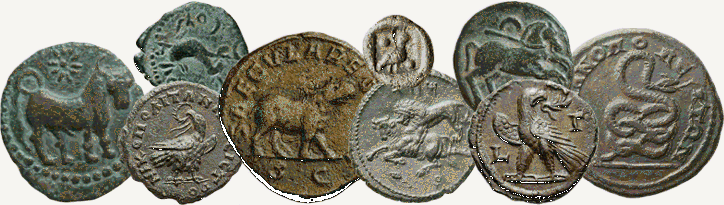
\includegraphics[width=\textwidth]{./media/coin.png}
	\caption{Antiguas monedas acuñadas.}
\end{imagen}

\section{El papel moneda y la bancarización}

Con el tiempo, las monedas de metal se volvieron difíciles de manejar en grandes cantidades, especialmente para las transacciones comerciales. Esto llevó al surgimiento del papel moneda. El uso del papel moneda se originó en China durante la dinastía Tang (618-907 d.C.), donde se utilizaba como recibo de depósitos de metales preciosos.

En Europa, el papel moneda fue introducido más tarde, principalmente por los bancos que emitían notas bancarias respaldadas por reservas de oro y plata. Estas notas podían ser intercambiadas por el valor equivalente en metales preciosos, lo que facilitó el comercio y el desarrollo de los mercados financieros.

\subsection{Cifras clave de la historia del dinero}

En el cuadro~\ref{moneyhistory}, se observan algunos eventos históricos clave en la evolución del dinero y sus correspondientes fechas.

\begin{table}[!ht]
\sf\footnotesize\setlength\tabcolsep{4pt}
\centering
\begin{tabular}{l | S[table-format=4.0]}
\toprule
\textbf{Evento} & \textbf{Año} \\
\midrule
Primera acuñación de monedas en Lidia & 700 \\
\midrule
Introducción del papel moneda en China & 618 \\
\midrule
Primera casa de moneda en Roma & 289 \\
\midrule
Establecimiento del patrón oro en el Reino Unido & 1821 \\
\midrule
Primera emisión de dólares en EEUU & 1792 \\
\midrule
Abolición del patrón oro & 1971 \\
\bottomrule
\end{tabular}
\caption{Eventos importantes en la historia del dinero.}\label{moneyhistory}
\end{table}

\section{La era digital y el futuro del dinero}

En la actualidad, el dinero ha dado un giro hacia lo digital. Las transacciones electrónicas han superado al uso de efectivo en muchas partes del mundo. Con la invención de las criptomonedas, como Bitcoin, estamos viendo una transformación aún más radical en cómo las personas perciben y utilizan el dinero.

Las criptomonedas son un tipo de dinero digital que utiliza la tecnología de \textit{blockchain} para garantizar transacciones seguras sin la necesidad de intermediarios como bancos o gobiernos. Aunque su uso todavía no está generalizado, las criptomonedas han generado un debate significativo sobre el futuro del dinero y los sistemas financieros.

\begin{figure}[!ht]
\begin{mdframed}[backgroundcolor=gray!5,linewidth=0.5pt]
\centering
\begin{tikzpicture}
% Axes
\draw[thick,->] (0,0) -- (5,0) node[right] {Año};
\draw[thick,->] (0,0) -- (0,5) node[above] {Uso de dinero digital (\%)};

% Data points
\draw[thick, color=blue] plot[smooth] coordinates {(0,0.5) (1,0.7) (2,1.2) (3,2.5) (4,4) (5,4.5)};

% Labels
\node at (0,0.3) {2000};
\node at (1,0.7) {2005};
\node at (2,1.2) {2010};
\node at (3,2.5) {2015};
\node at (4,4) {2020};
\node at (5,4.5) {2025};
\end{tikzpicture}
\end{mdframed}
\caption{Crecimiento del uso de dinero digital.}\label{monedas}
\end{figure}

\section{Conclusiones}

La evolución del dinero refleja no solo cambios en la tecnología y la economía, sino también en la sociedad y la cultura. Desde los primeros sistemas de trueque hasta las monedas digitales descentralizadas, el dinero ha sido un motor clave para el progreso humano. En el futuro, el dinero continuará evolucionando a medida que las nuevas tecnologías y modelos económicos surjan, cambiando la manera en que interactuamos con la economía global.



\backmatter

\chapter[\hspace{2pc}Referencias]{Referencias}
\printbibliography[heading=none]

\chaptermark{Índice de autoras y autores del aparato bibliográfico}
\addcontentsline{toc}{chapter}{\hspace{2pc}Índice de autoras y autores del aparato bibliográfico}

\Author{Índice de autoras y autores del aparato bibliográfico}
\raggedright
{\small
	\printindex[names]
}
\justifying

\chapter*{Colofón}

La composición tipográfica de este libro se realizó utilizando gbTeXpublisher.

Las familias tipográficas utilizadas dentro del libro son: IBM Plex, una superfamilia de tipografía abierta, diseñada y desarrollada conceptualmente por Mike Abbink en IBM con colaboración de Bold Monday y Libertinus, bifurcación de la fuente Linux Libertine, diseñada para el texto del cuerpo y la lectura extendida.


\newpage
\pagestyle{empty}
{\textcolor{white}{.}}

\end{document}
